\documentclass[11pt]{amsart}
%\documentclass[11pt]{report}
\usepackage[toc,page]{appendix}
\usepackage{float}
\usepackage{mathtools}
\usepackage{geometry}        % See geometry.pdf to learn the layout options.
\geometry{a4paper}           % ... or a4paper or a5paper or ...
%\geometry{landscape}        % Activate for for rotated page geometry
%\usepackage[parfill]{parskip} % Activate to begin paragraphs with empty line
\usepackage{graphicx}
\usepackage{amssymb}
\usepackage{epstopdf}

\usepackage[most]{tcolorbox}
\definecolor{block-gray}{gray}{0.85}
\newtcolorbox{myquote}{colback=block-gray,grow to right by=+0mm,grow to left by=-10mm, boxrule=0pt,boxsep=0pt,breakable}

\DeclareGraphicsRule{.tif}{png}{.png}{`convert #1 `dirname #1`/`basename #1 .tif`.png}
\graphicspath{ {images/} }

\renewcommand{\familydefault}{\sfdefault}
\newcounter{defctr}

\title{PEG Security}
\author{Kees-Jan Hermans}
%\date{}                     % Activate to display a given date or no date

\begin{document}
\maketitle

This document contains a description of the measures that
where implemented in the open source software Parsing Expression
Grammar (PEG) suite Naigama,
with the express intent to (more) securely enable
parsing and processing of inputs.

\vspace*{3\baselineskip}

\begin{figure}[H]
\centering
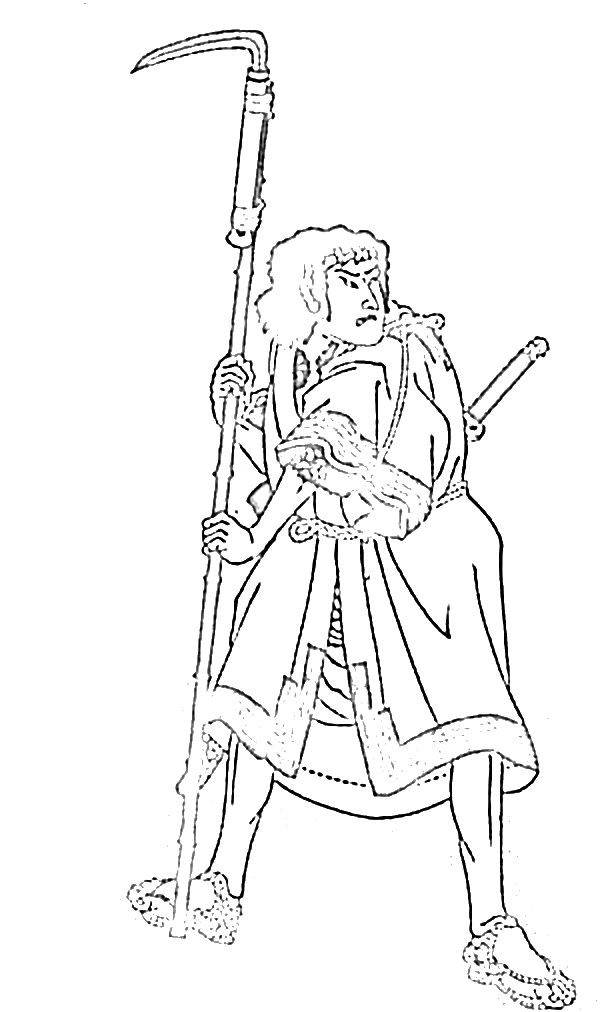
\includegraphics[width=60mm]{../naigama}
\end{figure}

\vfill

\begin{table}[]
\centering
\begin{tabular}{ll}
Author & Kees-Jan Hermans / kees.jan.hermans@gmail.com \\
Version & 0.1.2 \\
Classification & - \\
Generated on & \today \\
\end{tabular}
\end{table}

\newpage

\tableofcontents

\setlength{\parindent}{4em}
\setlength{\parskip}{1em}

\newpage
\section{Rationale}

In the whitepapers of Ierusalemschi et al \cite{bib:peg}
on Parsing Expression Grammars,
an assembly language is proposed that grammar is
compiled to, transforming a potentially infinitely deep structure
description into a list of instructions, allowing a simple state machine
with an endless loop to execute what would otherwise require 
ecursion in the execution of the parser.

It's a simple, elegant, efficient and secure concept:
with somewhere around 20 instructions, one can
formulate all conditions that a (text) parser could encounter
to a relatively deep level of syntactic understanding (even down
to such things as dynamically matching open- and closing XML tags,
for example).

This assembly language's instructions however,
oftentimes perform a combination of underlying manipulations of the
state machine, of which many make a repeated appearance.
For example, the \texttt{commit $<$label$>$} instruction is assumed to
perform the following steps:

\begin{itemize}
\item Pop a 'choice' element off the stack (must be the top element).
\item Jump to $<$label$>$
\end{itemize}

Where the \texttt{FAIL} condition (and the \texttt{fail} instruction)
is assumed to:

\begin{itemize}
\item Pop any item that isn't a 'choice' element off the stack.
\item Pop a 'choice' element off the stack (must now be the top element).
\item Recreate the machine state stored in that element.
\item Jump to the offset stored in that element.
\end{itemize}

And the \texttt{partialcommit $<$label$>$} instruction is assumed to
 \footnote{The expansion of the 'partialcommit' instruction has been purposely
worded in a convoluted manner; the original paper means the 'partialcommit'
as an optimization, where the 'choice' element on the stack isn't popped
and subsequently pushed, but \textit{updated}. In this paper, I propose
a different model of stack, that allows for efficient popping and pushing.}
:

\begin{itemize}
\item Pop a 'choice' element off the stack (must be the top element).
\item Update the input position in the machine state stored in that element.
\item Push the 'choice' element back on the stack.
\item Jump to $<$label$>$
\end{itemize}

However, if we look at the way all these instructions are conceptualised,
we can see a lot of similarities: the stack is pushed onto, and popped from,
the input position is guarded and increased, and there are jumps.
These should all be familiar to people who know 'proper' assembly
languages such as i386 or ARM. Note that the goal of this paper is not
to promote compiling down to an \textit{actual} assembly language, but
rather to one that is still abstract, but has more similarities with
those assembly languages.

Wouldn't it be worth exploring, then,
if the 'sub instructions' were somehow made more concrete, and actually
compile a PEG not to the whitepaper's assembly language, but to one that
is more elementary? Let's explore the arguments as to why this could be so.
That is to say: why pursuing another, 'deeper' assembly for PEG's could be
beneficial.

\begin{itemize}
\item For one, 'deeper', more 'CPU like' assembly instructions can be monitored
more ...
\item There could be (even) fewer of them.
\item And it could yield faster and / or yield better optimizations and
thereafter be faster.
\item Hardware implementations of the machine could be easier to implement.
\end{itemize}

The obvious downsides, from a first glance, would be:
The bytecode would be bigger; the original bytecode is also a means to
compress functional logic. The upside to that is that the machine size
would be smaller.
More elementary instructions also lack security, because they lack more
context in which their monitoring could take place.
Forensics, trying to discover why a piece of grammar would yield a
certain piece of bytecode, would be more difficult.

\section{Threat Model}
Assuming that the Naigama parser, like many parsers, implements the
following workflow sequence:

\begin{itemize}
\item A policy that comprehensively describes the structure
      of a piece of input data is written down in a grammar.
\item The grammar is held against
      a piece of real input data by an engine (via, in this case,
      a process of compilation and assembly to a bytecode).
\item The engine provides a conclusion: the real
      input data either matches the grammar or it doesn't.
\item Optional detail of matching inputs follow, or subsequent actions
      are performed on the input.
\end{itemize}

This paper then proposes that a parser is threatened by the following phenomena
(apart from malicious inputs, or inputs which have been changed before being
offered to the engine, which are considered
an elementary form of protection that a parser should offer):

\refstepcounter{defctr}
\newcounter{threatintent} \setcounter{threatintent}{\value{defctr}}
\thedefctr .
The intention of the grammar writer is not easily conveyed in bytecode
(and is therefore prone to mistakes).

The intention of the grammar writer is not correctly conveyed in
bytecode, and:

\refstepcounter{defctr}
\newcounter{threatbcerror} \setcounter{threatbcerror}{\value{defctr}}
\thedefctr .
This is something that can be proven before execution.

\refstepcounter{defctr}
\newcounter{threatbcexec} \setcounter{threatbcexec}{\value{defctr}}
\thedefctr .
This only becomes apparent during execution.

The intention of the grammar writer is correctly conveyed in bytecode,
but the bytecode is somehow corrupted, because either:

\refstepcounter{defctr}
\newcounter{threatbcsign} \setcounter{threatbcsign}{\value{defctr}}
\thedefctr .
The bytecode is replaced by a malicious or stupid actor before execution, or

\refstepcounter{defctr}
\newcounter{threatbcupset} \setcounter{threatbcupset}{\value{defctr}}
\thedefctr .
Some of the bytecode's bits accidentally change value before or
during execution.

\refstepcounter{defctr}
\newcounter{threatengine} \setcounter{threatengine}{\value{defctr}}
\thedefctr .
The intention of the grammar writer is correctly conveyed in bytecode,
but the engine is somehow corrupted during execution.

\refstepcounter{defctr}
\newcounter{threatinput} \setcounter{threatinput}{\value{defctr}}
\thedefctr .
The input is somehow corrupted during execution.

\section{Easy Pickings and Assumptions}

\subsection{Coveying the Intention of the Grammar Writer}

Wrt [Threat \thethreatintent], it is assumed that the grammar writer has been
or can be taught to use Regular Expressions \cite{bib:regex}, and
Backus-Naur (-like) notation \cite{bib:backusnaur}. These are the fundamentals
behind PEG grammar notation when it comes to defining rule terminals and
non terminals respectively (as well as PEG specific details, like left
recursion being forbidden, etc).

It is also assumed, should this not be the case, that for example, a GUI
based policy definition application, exists or can be made. This document
does not deal with the specifics of those.

\subsection{The Hardness of the Bytecode Execution Engine}

Wrt [Threat \thethreatengine], it is assumed that a bytecode execution
engine can be ported to hardware (or a hardware description language, such
as VHDL \cite{bib:vhdl})  with relative ease. This is at least
intuitively supported by the following facts:

\begin{itemize}
\item The amount of bytecode instructions is relatively low (around thirty,
      many of which are only emitted by the optimizer, which is a step
      that can be skipped). See table [Table \ref{tab:naig_bytecode}]
      for all Naigama parser instructions.
\item The amount of memory manipulations that must be performed per
      bytecode instruction is relatively low. For reference, the Naigama
      bytecode engine main loop consists of about 400 lines of C code
      [src/gen2/lib/engine/naie\_engine\_loop.c].
\end{itemize}

Hardware execution of the PEG bytecode engine should provide some
confidence the risk of bitfaults or attacks on the engine logic itself, can
be considered minimal [citation needed].

\section{Measures}
\subsection{Measure: Modularization of Toolchain}

\subsubsection{Modules}
Naigama cuts the process of parsing into five potential stages, each with
their respective inputs and outputs. Outputs of a stage acts as input
for the next. The stages / modules are:

\begin{itemize}
\item{Compiler. Takes grammar as input and outputs assembly.}
\item{Optimizer. Takes assembly as input and outputs (optimized) assembly.}
\item{Assembler. Takes assembly as input and outputs bytecode.}
\item{Engine. Takes bytecode and the input and outputs the action list.}
\item{Action Processor. Executes the action list on the input.}
\end{itemize}

On top of this, Naigama also provides a disassembler (to verify that
the bytecode produced by the assembler is actually being produced correctly).

Advantages of modularization are:

\begin{itemize}
\item{Drop in replacements. For example, if one does't trust the compiler
      per se, one can introduce only another compiler, without having to
      recreate the entire toolchain.}
\item{Foregoing modules, for example:}
  \begin{itemize}
  \item{Write assembly from scratch (and forego the compiler, or have
        another type of compiler altogether (for example, P4 \cite{bib:p4})).}
  \item{Make the use of the optimizer optional (for example, to check
        whether optimized and unoptimized assembly yields the same results
        on an input).}
  \item{Forego the use of the action processor, when you know there aren't
        any actions to process (matching inputs is fine in itself).}
  \end{itemize}
\item{Reversing the output of modules. Bytecode can be reduced to assembly
      by the disassembler. Other reversals are under study.}
\end{itemize}

Modularization addresses [Threat \thethreatbcerror], by allowing modules
to be replaced, foregone and / or reversed, making the process by which
the intention of the person drafting policy is converted into bytecode,
more free and more transparent.

LPEG \cite{bib:lpeg} by contrast, compiles directly from grammar to bytecode,
but can yield a decompiled assembly output in debug mode
[lpprint.c, which requires LPEG\_DEBUG to be \#defined.] This assembly
however, can not be re-introduced into the chain.

\subsubsection{Artefact: Slot Map}
The Naigama compiler can be instructed to emit a secondary file called
the slot map. This file contains a mapping from 'intuitive' (that is,
derived from rule names and textual data from the production definition)
to slot numbers of capture regions that the
compiler encountered during its pass over the grammar.

A slot map enables the developer to use names for capture regions instead
of index numbers (which can shift when the grammar is rewritten), possibly
preventing mistakes in Naigama library using code.

\subsubsection{Artefact: Label Map}
The Naigama assembler can be instructed to emit a secondary file called
the label map. This file contains a mapping from label names, as created
by the compiler, to their offsets in the bytecode.

A label map allows for better debugging, as offsets in the bytecode
can be reduced to more intuitively named labels.

\subsubsection{Tooling: Disassembler}

Naigama comes with a disassembler (in ./bin/disassembler), which recreates
the Naigama assembly from bytecode. The output of the disassembler prefixes
all instructions with a label, consisting of its offset in the bytecode,
in decimal (the reason that labels may start with a number in Naigama).

\subsubsection{Tooling: Debugger}

The Naigama engine can be run in debugging mode. In this case, one can
interactively step through the parsing process, instruction by instruction,
and when the FAIL state is invoked.

\begin{myquote}
\begin{verbatim}
$ ./src/gen2/main/engine/naie \
  -c ./src/gen1/grammar/grammar.byc \
  -l ./src/gen1/grammar/grammar.byc.labelmap \
  -i ./src/gen1/grammar/grammar.naig \
  -di 0 -v

\end{verbatim}
\end{myquote}
\textit{Example of the invocation of the Naigama engine as debugger.}


\subsection{Measure: Read-only-ness of Input and Bytecode}

The design of the modules that make up the Naigama parser system is such,
that inputs and bytecode are always considered read-only, allowing them to
be read from places that enforce this quality in something that is better
protected from modification than a kernel's flags on certain regions of
RAM.

Should it be necessary to make modifications to the input, then only in
the last module or stage of the process - the action processor - a copy
of the input can be made in read-write memory.

Read-onlyness of the memories used for storing inputs and bytecode, addresses
[Threat \thethreatbcupset] and [Threat \thethreatinput].

\subsection{Measure: Alignment and Length of Instructions}

\subsubsection{General Alignment on 32 bit Boundaries}

All bytecode, as emitted by the assembler, has the beginning of its
instructions aligned on 32 bit boundaries. This allows one to detect
a bit fault in the least two significant bits of any offset: they should 
always be zero.

\subsubsection{Instruction Length}

The length of an instruction is:

\begin{itemize}
\item Fixed. That is to say: there are no variable length instructions.
The length of the instruction is given by the opcode.
\item Encoded in the instruction opcode itself. That is to say: the
second most relevant byte contains the length of the instruction, minus
the length of the opcode (which is always four).
\end{itemize}

Instruction alignment addresses [Threat \thethreatbcupset].

\subsection{Measure: Instruction Opcode Hamming Distance}

Naigama bytecode Instruction opcdes are chosen in such a manner
that it takes at least two bit flips for one instruction to be
possibly confused for another (Hamming Distance is always greater than,
or equal to two).

LPEG \cite{bib:lpeg} by contrast, uses a simple enum for the
opcode values [lpvm.h line 12].

[Table \ref{tab:naig_bytecode}] lists all Naigama parser
instructions with their opcode values.

The introduction of Hamming distance in Naigama bytecode instruction
opcode values addresses [Threat \thethreatbcupset].


%\begin{table}[]
\begin{center}
\caption{Naigama Bytecode Instructions}
\label{tab:naig_bytecode}
\begin{longtable}{lllll}
\textbf{Mnemonic} & \textbf{Opcode} & \textbf{Param1} & \textbf{Param2} & \textbf{Length} \\
\endhead
any & 000003e4 &  &   & 4 \\
backcommit & 000403c0 & address &   & 8 \\
call & 00040382 & address &   & 8 \\
catch & 00040393 & address &   & 8 \\
char & 000403d7 & char &   & 8 \\
closecapture & 00040300 & slot &   & 8 \\
commit & 00040336 & address &   & 8 \\
condjump & 00080321 & register & address  & 12 \\
counter & 00080356 & register & value  & 12 \\
end & 000400d8 & code &   & 8 \\
endisolate & 00003005 &  &   & 4 \\
endreplace & 00000399 &  &   & 4 \\
fail & 0000034b &  &   & 4 \\
failtwice & 00000390 &  &   & 4 \\
intrpcapture & 0008000f &  &   & 12 \\
isolate & 00043003 & slot &   & 8 \\
jump & 00040333 & address &   & 8 \\
maskedchar & 00080365 & char & mask  & 12 \\
mode & 0004000a &  &   & 8 \\
noop & 00000000 &  &   & 4 \\
opencapture & 0004039c & slot &   & 8 \\
partialcommit & 000403b4 & address &   & 8 \\
quad & 0004037e & quad &   & 8 \\
range & 000803bd & from & until  & 12 \\
replace & 00080348 & slot & address  & 12 \\
ret & 000003a0 &  &   & 4 \\
scr\_add & 0000050c &  &   & 4 \\
scr\_array & 00040006 &  &   & 8 \\
scr\_assign & 000005c9 &  &   & 4 \\
scr\_bitand & 00000527 &  &   & 4 \\
scr\_bitnot & 00000574 &  &   & 4 \\
scr\_bitor & 0000053c &  &   & 4 \\
scr\_bitxor & 0000052d &  &   & 4 \\
scr\_builtin & 000407cf &  &   & 8 \\
scr\_call & 00040503 &  &   & 8 \\
scr\_condjump & 0004000c &  &   & 8 \\
scr\_dec & 0000053a &  &   & 4 \\
scr\_div & 00000581 &  &   & 4 \\
scr\_equals & 0000056c &  &   & 4 \\
scr\_gt & 0000056f &  &   & 4 \\
scr\_gteq & 0000054d &  &   & 4 \\
scr\_inc & 000005f6 &  &   & 4 \\
scr\_index & 00000009 &  &   & 4 \\
scr\_logand & 0000052e &  &   & 4 \\
scr\_lognot & 000005f9 &  &   & 4 \\
scr\_logor & 000005a9 &  &   & 4 \\
scr\_lt & 00000595 &  &   & 4 \\
scr\_lteq & 00000522 &  &   & 4 \\
scr\_mul & 0000058b &  &   & 4 \\
scr\_nequals & 00000572 &  &   & 4 \\
scr\_pop & 000005cc &  &   & 4 \\
scr\_pow & 00000542 &  &   & 4 \\
scr\_push & 000c0003 &  &   & 16 \\
scr\_ret & 00000555 &  &   & 4 \\
scr\_shift & 00040005 &  &   & 8 \\
scr\_shiftin & 0000057d &  &   & 4 \\
scr\_shiftout & 00000517 &  &   & 4 \\
scr\_string & 000017bb &  &   & 4 \\
scr\_sub & 000005bb &  &   & 4 \\
set & 002003ca & set &   & 36 \\
skip & 00040330 & number &   & 8 \\
span & 002003e1 & set &   & 36 \\
testany & 00040306 & address &   & 8 \\
testchar & 0008039a & address & char  & 12 \\
testquad & 000803db & address & quad  & 12 \\
testset & 00240363 & address & set  & 40 \\
trap & ff00ffff &  &   & 4 \\
var & 000403ee & slot &   & 8 \\
\end{longtable}
\end{center}
%\end{table}


\subsection{Measure: Randomization of Opcode Values}

The source code base allows you to re-randomize the instruction set.
You can do this by issueing 'make instructions'. This will upset
your entire build tree and lock you out from previous versions
of instruction sets and bytecodes generated therein.

It is a roadmap item currently to generate a file format for bytecode
that comes with an 'instruction set signature' that allows engine
to recognize or reject non conforming bytecodes.

\subsection{Measure: Traps}
\label{sec:traps}

\subsubsection{Addition of the 'Trap' Instruction}

One or more 'trap' instructions can be emitted by the compiler in places that,
under normal circumstances, would be unreachable. For example, straight
after the following possible instructions:

\begin{itemize}
\item{jump}
\item{ret}
\item{end}
\item{commit}
\item{partialcommit}
\item{backcommit}
\item{fail}
\item{failtwice}
\end{itemize}

The possible advantage of placing traps is that, when the value of the
bytecode offset in the engine is somehow subverted, it may land on a trap
and halt execution.

The addition of the 'trap' instruction addresses [Threat \thethreatbcupset].

\input{measure_fileformat.tex}
\subsection{Measure: Endless Loop Detection}

Endless loop detection can be done in two places: while compiling the
grammar, and while running the bytecode in the engine.

\subsubsection{Endless Loop Detection During Compilation}

Since PEG is a left recursive parser, it explicitly forbids
leftmost recursion. Rules that reference themselves as the first item
in their production definition, like so:

\begin{myquote}
\begin{verbatim}
RULE <- RULE OTHER_RULE_OR_TERMINAL

\end{verbatim}
\end{myquote}

will necessarily create an endless loop when encountered during execution,
and are therefore forbidden by the compiler. However, it's quite easy to
create second, third or n-th order offences. For example:

\begin{myquote}
\begin{verbatim}
RULE1 <- RULE2 'blah'
RULE2 <- RULE1 'foo'

\end{verbatim}
\end{myquote}

will wreak the same havoc, but is less easy to detect by the compiler.

\subsubsection{Endless Loop Detection During Execution}

Endless loop detection in both LPEG and Naigama is a fairly straightforward
process in the engine: the second time the engine encounters the same
combination of input offset value and bytecode offset value, is when the
code is caught in an endless loop, and the execution will halt with a
system error.

Endless loop detection addresses [Threat \thethreatbcexec] and
[Threat \thethreatbcerror].

\subsection{Error Handling}

Naigama knows three types of error condition:

\begin{itemize}
\item No match: a FAIL condition was encountered, and there was no 'catch' stack
element to divert the bytecode offset to an alternative path of execution,
rolling up the entire stack.
\item Bytecode error: an endless loop or trap instruction was encountered.
The latter is intended to catch errors of the third type (bytecode corruption),
but the engine cannot know that it has not been intentionally directed to
encounter this instruction.
\item Bytecode corruption: misalignment, bad instruction, pointers outside
the bytecode memory area all lead to immediate halting of execution.
\end{itemize}

%\section{Consideration: Unicode}

\subsection{Unicode Grammar}

\subsection{Unicode Input}

The following grammar:

\begin{myquote}
\begin{verbatim}
UTF8TEXT    <- UTF8CHAR* !.
UTF8CHAR    <- ASCII / DOUBLE / TRIPLE / QUADRUPLE
ASCII       <- [\000-\177]
DOUBLE      <- [\300-\337] [\200-\277]
TRIPLE      <- [\340-\357] [\200-\277] [\200-\277]
QUADRUPLE   <- [\360-\367] [\200-\277] [\200-\277] [\200-\277]

\end{verbatim}
\end{myquote}
\textit{Example of a xxx}


\section{Conclusion}

[Threat \thethreatintent] is not addressed by Naigama. It is assumed that
the the grammar syntax is intuitive enough for the
person drafting policy. Otherwise, it is assumed that a GUI application
exists which can make this task easier.

[Threat \thethreatbcerror] is addressed by modularization of the Naigama
toolchain, allowing replacement, foregoing and reversing of modules and / or
their function. Debugging and fuzzing, both roadmap items, should make the
toolchain more complete.

[Threat \thethreatbcexec] is addressed by endless loop detection.

However, intuitively, it seems as if more could be done here.
Debugging could play a role, as well as several other, perhaps
more 'artificially intelligent' options (for example, when the stack
grows in size to far beyond the amount of bytes in input).

[Threat \thethreatbcsign] is not yet addressed by Naigama. This is in
the roadmap section (secure file format).

[Threat \thethreatbcupset] is addressed by the Hamming distance of
opcodes, the alignment of instructions, and the possibility to insert
trap instructions in the bytecode.

[Threat \thethreatengine] is only addressed by Naigama in the sense that
it intuitively seems to be well placed for implementation
in hardware.

[Threat \thethreatinput] is addressed by Naigama by strictly enforcing
the read-only-ness of bytecode and input.

\section{Roadmap}

\subsection{Fuzzing}

Apart from endless recursion in inputs, and straight quantifiers with
an indefinite upper bound (which should be given reasonable limits by
the fuzzer), the PEG grammar and bytecode structure as such (essentially:
one byte at a time, you always know what's coming, alternative paths are
not attempted), make it eminently usable to create fuzzed inputs to the engine.

A fuzzer would be a great tool to verify whether the intention of the
policy designer is met
(as well as a great test for the strength of the engine).

\subsection{Debugging}

This item should be addressed by the introduction of a checkpoint instruction
that is emitted only in bytecodes that are marked for debugging, and that
trigger the debugging engine to halt execution and allow stepping from that
point onward. The use of label and slot maps, already in place, should allow
for intuitive feedback to the debugger user at that point.

Alternatively, the engine is provided with a command line option that
instructs it to halt on a given bytecode offset.

\subsection{Bytecode Transport File Format}

A bytecode format with a cryptography based authentication string (HMAC)
or digital signature, is currently defined.


\newpage
\section{Colofon}
\listoftables
\begin{thebibliography}{12}

\bibitem{bib:peg}
  A Text Pattern-Matching Tool based on Parsing Expression Grammars
  https://www.inf.puc-rio.br/\textasciitilde roberto/docs/peg.pdf

\bibitem{bib:regex}
  Regular Expressions
  https://en.wikipedia.org/wiki/Regular\_expression

\bibitem{bib:backusnaur}
  Backus Naur Form
  https://en.wikipedia.org/wiki/Backus-Naur\_form

\bibitem{bib:yacc}
  Yacc Yet Another Compiler Compiler
  https://en.wikipedia.org/wiki/Yacc

\bibitem{bib:javascript}
  JavaScript, or ECMAScript
  https://www.ecma-international.org/publications/standards/Ecma-262.htm

\bibitem{bib:json}
  JSON, JavaScript Object Notation
  https://www.json.org/

\bibitem{bib:perl}
  Perl, the Perl Programming Language
  https://www.perl.org/

\end{thebibliography}


\newpage
\begin{appendices}
\section{Finding: Bitfault Checking Mechanisms}

\subsection{The Simple Case}

The following grammar:

\begin{myquote}
\begin{verbatim}
DATA <- .+

\end{verbatim}
\end{myquote}

Yielding the following assembly:

\begin{myquote}
\begin{verbatim}
0: call 20
8: end 0
16: any
20: catch 40
28: any
32: partialcommit 28
40: ret
44: end 0

\end{verbatim}
\end{myquote}

Undergoes a sequential single bit toggle for each bit of the resulting
bytecode. The engine is fed a happy flow (short) piece of data
(in the case of this grammar, any data will do).
Ideally, the engine would always detect this and return an
error representing that. However, the engine as it stands, sometimes
returns zero (no error). The result of all bitflips are listed below
(416 bits total in the bytecode, Naigama version 0.3.6):

\begin{myquote}
\begin{verbatim}
Code   0 occurence 99   // success
Code -19 occurence 3    // stack corruption
Code -20 occurence 209  // bad opcode
Code -21 occurence 104  // overflow (jump out of bounds)
Code -32 occurence 1    // endless loop

\end{verbatim}
\end{myquote}

This seems like a lot of successful exits, however, there are two unchecked
'end' instructions with a 32 bit parameter (end code), and also: the second
'end' instruction is completely out of reach, so 96 of the 99 successful
exits are still quite harmless.

\begin{myquote}
\begin{verbatim}
-- Bit 96
0: call 16
8: end 16777216
16: any
20: catch 40
28: any
32: partialcommit 28
40: ret
44: end 0

\end{verbatim}
\end{myquote}
\textit{Example of a 'harmless' bit flip}

The remaining three mess up, because they change jump instructions
which accidentally end up well enough:

\begin{myquote}
\begin{verbatim}
-- Bit 58
0: call 20
8: end 0
16: any
20: catch 40
28: any
32: partialcommit 28
40: ret
44: end 0

\end{verbatim}
\end{myquote}

Here, the offset in the 'call' instruction is changed from 16 to 20, passing
the 'any' instruction, going directly into the endless loop, making this
bytecode equivalent to '.*' instead of '.+'.

\begin{myquote}
\begin{verbatim}
-- Bit 218
0: call 16
8: end 0
16: any
20: catch 44
28: any
32: partialcommit 28
40: ret
44: end 0

\end{verbatim}
\end{myquote}

Here, the offset in the 'catch' instruction is changed from 40 to 44,
jumping to the last 'end' instruction instead of to the 'ret' instruction.
The net effect is the same.

\begin{myquote}
\begin{verbatim}
-- Bit 221
0: call 16
8: end 0
16: any
20: catch 8
28: any
32: partialcommit 28
40: ret
44: end 0

\end{verbatim}
\end{myquote}

Here, the offset in the 'catch' instruction is changed from 40 to 8,
jumping to the first 'end' instruction instead of to the 'ret' instruction.
The net effect is the same.

\subsection{A More Complex Case}

The following grammar:

\begin{myquote}
\begin{verbatim}
JSON         <- %s* HASH %s*
HASH         <- '{' %s* OPTHASHELTS %s* '}'
OPTHASHELTS  <- HASHELTS / ...
HASHELTS     <- HASHELT %s* ',' %s* HASHELTS / HASHELT
HASHELT      <- STRING %s* ':' %s* VALUE
ARRAY        <- '[' %s* OPTARRAYELTS %s* ']'
OPTARRAYELTS <- ARRAYELTS / ...
ARRAYELTS    <- VALUE %s* ',' %s* ARRAYELTS / VALUE
VALUE        <- STRING / FLOAT / INT / BOOL / NULL / HASH / ARRAY
STRING       <- { '"' [^"]* '"' }
INT          <- { [0-9]+ }
FLOAT        <- { [0-9]* '.' [0-9]+ }
BOOL         <- { 'true' / 'false' }
NULL         <- { 'null' }

\end{verbatim}
\end{myquote}

With a JSON input that touches on all of the grammar's aspects:

\begin{myquote}
\begin{verbatim}
{"widget": {
    "debug": true,
    "window": {
        "title": "Sample Konfabulator Widget",
        "name": "main_window",
        "width": 500,
        "height": 500
    },
    "image": {
        "src": { "foo" : "bar", "bar" : 0.23 },
        "name": "sun1",
        "hOffset": 250.0,
        "vOffset": 250.5,
        "alignment": "center"
    },
    "text": {
        "data": [ "some", "sub", "array", 3, 5.7, false, null ],
        "size": 36,
        "style": null,
        "name": "text1",
        "hOffset": 250,
        "vOffset": 100,
        "alignment": "center",
        "onMouseUp": "sun1.opacity = (sun1.opacity / 100) * 90;"
    }
}}

\end{verbatim}
\end{myquote}

Will yield the following statistics wrt exit codes:

\begin{myquote}
\begin{verbatim}
Code   1 occurence 437   // parser failure
Code   0 occurence 5044  // success
Code -19 occurence 144   // stack corruption
Code -20 occurence 4521  // bad opcode
Code -21 occurence 1603  // overflow
Code -23 occurence 322   // action list
Code -32 occurence 25    // endless loop
                  -----+
                  12096

\end{verbatim}
\end{myquote}

The amount of parser failures is explainable: this bytecode contains
a large amount of sets. Sets are 32 bytes long and a bitflip in them
can cause both false positives and false negatives in parsing, making
the engine exit as if the input had been incorrect. However, most bitflips
in bytecode sets will not result in a failure at all: since most of the
bits in most sets are zero, and this case tests a happy flow, most sets
will only become more, but unnoticedly, 'inclusive'.

This is the major reason for the large amount of successful exits.

Now we run the compiler with traps. The result:

\begin{myquote}
\begin{verbatim}
Code   0 occurence 1     // success
Code -19 occurence 3     // stack corruption
Code -20 occurence 70    // bad opcode
Code -21 occurence 21    // overflow
Code -29 occurence 12896 // trap
Code -32 occurence 1     // endless loop
                   ----+
                   12992

\end{verbatim}
\end{myquote}

The result is rather dramatic. There are more instructions (7\%) in the bytecode
(this compiler generates traps before and after the assembly for each rule only,
but could emit a lot more of them (see [Section \ref{sec:traps}]))
but the amount of successful exits decreases to almost zero.

In fact, the only successful change comes when 'call 16' at offset zero
is changed to 'call 272', and at offset 272 we find a 'ret' instruction.

\section{Addition: Prefix Rule}

Consider the difference between the following two JSON grammar
definitions:

\begin{myquote}
\begin{verbatim}
JSON         <- %s* HASH %s* END
HASH         <- CBOPEN %s* OPTHASHELTS %s* CBCLOSE
OPTHASHELTS  <- HASHELTS / ...
HASHELTS     <- HASHELT %s* COMMA %s* HASHELTS / HASHELT
HASHELT      <- STRING %s* COLON %s* VALUE
ARRAY        <- ABOPEN %s* OPTARRAYELTS %s* ABCLOSE
OPTARRAYELTS <- ARRAYELTS / ...
ARRAYELTS    <- VALUE %s* COMMA %s* ARRAYELTS / VALUE
VALUE        <- STRING / INT / FLOAT / BOOL / NULL / HASH / ARRAY
STRING       <- { '"' ( '\\' ([nrtv"] / [0-9]^3) / [^"\\] )* '"' }
INT          <- { [0-9]+ }
FLOAT        <- { [0-9]* '.' [0-9]+ }
BOOL         <- { 'true' / 'false' }
NULL         <- { 'null' }
CBOPEN       <- '{'
CBCLOSE      <- '}'
ABOPEN       <- '['
ABCLOSE      <- ']'
COMMA        <- ','
COLON        <- ':'
END          <- !.

\end{verbatim}
\end{myquote}
\textit{Example of JSON grammar definition with explicit optional whitespace skipping}

\begin{myquote}
\begin{verbatim}
TOP          <- JSON
__prefix     <- %s*
JSON         <- HASH END
HASH         <- CBOPEN OPTHASHELTS CBCLOSE
OPTHASHELTS  <- HASHELTS / ...
HASHELTS     <- HASHELT COMMA HASHELTS / HASHELT
HASHELT      <- STRING COLON VALUE
ARRAY        <- ABOPEN OPTARRAYELTS ABCLOSE
OPTARRAYELTS <- ARRAYELTS / ...
ARRAYELTS    <- VALUE COMMA ARRAYELTS / VALUE
VALUE        <- STRING / FLOAT / INT / BOOL / NULL / HASH / ARRAY
STRING       <- { '"' ( '\\' ([nrtv"] / [0-9]^3) / [^"\\] )* '"' }
INT          <- { [0-9]+ }
FLOAT        <- { [0-9]* '.' [0-9]+ }
BOOL         <- { 'true' / 'false' }
NULL         <- { 'null' }
CBOPEN       <- '{'
CBCLOSE      <- '}'
ABOPEN       <- '['
ABCLOSE      <- ']'
COMMA        <- ','
COLON        <- ':'
END          <- !.

\end{verbatim}
\end{myquote}
\textit{Example of JSON grammar definition with implicit optional whitespace skipping}

The latter grammar definition is a bit longer (it makes a jump across the '\_\_prefix'
rule definition), but is much more readable with the clutter of optional whitespace
matchers removed. The rule defined as '\_\_prefix' takes care of that.

The prefix rule is a rule that is always called and executed
before the rest of the production logic of any of the rules
that are defines after it in a grammar.

\section{Counters}

An addition that the Naigama makes to LPEG, is the introduction
of counters to prevent matchers being written out completely
when a large, but absolute, upper bound of a matcher's quantifier
is given.

For example:

\begin{myquote}
\begin{verbatim}
HEXLITERAL <- [0-9a-fA-F]^8-32

\end{verbatim}
\end{myquote}

Must be written out by LPEG as repetitions, like so:

\begin{myquote}
\begin{verbatim}
  set 000000000000ff037e0000007e000000000000000000000000000 ...
  set 000000000000ff037e0000007e000000000000000000000000000 ...
  set 000000000000ff037e0000007e000000000000000000000000000 ...
-- ... repeated eight times total ...

  set 000000000000ff037e0000007e000000000000000000000000000 ...
  partialcommit LABEL1
LABEL1:
-- ... repeated 24 times ...

\end{verbatim}
\end{myquote}

Naigama solves this by introducing counters. These are numbered
registers for a counter, whose value can only go down (to zero).
The instructions to implement a counted loop are
'counter' and 'condjump'. The first one sets the counter's value,
the second one only jumps when the value is non zero.
The grammar above is then compiled as follows:

\begin{myquote}
\begin{verbatim}
  call HEXLITERAL
  end
-- Rule
HEXLITERAL:
  counter 0 8
__TERM_2:
  set 000000000000ff037e0000007e000000000000000000000000000 ...
  condjump 0 __TERM_2
  catch __TERM_3
  counter 1 24
__TERM_4:
  set 000000000000ff037e0000007e000000000000000000000000000 ...
  partialcommit __TERM_5
__TERM_5:
  condjump 1 __TERM_4
  commit __TERM_3
__TERM_3:
  ret

\end{verbatim}
\end{myquote}

Not only delivers this feature much more efficient code, the code
is also less cluttered, and more de-compileable.

\end{appendices}

\end{document}
